\documentclass[12pt]{article}
\DeclareMathSizes{12}{13.5}{11}{12}
\usepackage[utf8]{inputenc}
\usepackage[margin=1.5cm]{geometry}
\usepackage{amsmath}
\usepackage{amssymb}
\usepackage{cancel}
\usepackage{graphicx}

\begin{document}
\section*{LEZIONE 6: CONDIZIONAMENTO DELLE FUNZIONI, \\ PROPAGAZIONE DEGLI ERRORI}
In questa lezione ci occuperemo di due aspetti importanti del calcolo approssimato, tramite esempi: l'effetto degli errori sulla variabile x e degli errori di arrotondamento nel calcolo dei valori di una funzione $f(x)$, e l'effetto degli errori di arrotondamento in un algoritmo iterativo che costruisce i valori di una successione convergente alla quantità da approssimare.\\
Cominciamo col calcolo di funzioni, visto che in pratica tutte le quantità utilizzate nel calcolo sono approssimate, possiamo innanzitutto porci la seguente domanda: qual è l'effetto sul valore di $f$ di un errore sulla variabile indipendente $x$?\\
Come sempre, siamo maggiormente interessati agli errori relativi. Consideriamo una funzione $f: I \mapsto \mathbb{R}$ dove I è un intervallo e $x, \tilde{x} \in I$ dove $\tilde{x} \approx x, x \neq 0$ con errore relativo\\
$\varepsilon_x = \frac{|x-\tilde{x}|}{|x|}$
cerchiamo di stimare $\varepsilon_{f(x)}$\\
\begin{equation}
    \varepsilon_{f(x)} = \frac{|f(x)-f(\tilde{x})|}{|f(x)|}, f(x) \neq 0
\end{equation}
supponendo f derivabile in I possiamo utilizzare la formula
di Taylor al primo ordine centrata in x
\begin{equation}
        f(\tilde{x}) \approx f(x) + f'(x)\cdot (\tilde{x}-x)
\end{equation}
da cui ricaviamo
\begin{equation}
        f(\tilde{x})-f(x) \approx f'(x)\cdot (\tilde{x}-x) \iff
        \frac{|f(\tilde{x})-f(x)|}{|f(x)|} \approx \frac{|f'(x)|}{|f(x)|} \cdot |\tilde{x}-x| = \frac{|f'(x)| \cdot |x|}{|f(x)|} \cdot \frac{|\tilde{x}-x|}{|x|}
\end{equation}
che possiamo riassumere con $\varepsilon_{f(x)} \approx condf(x) \varepsilon_x$ dove
\begin{equation}
    condf(x)=\frac{|f'(x)|\cdot|x|}{|f(x)|}
\end{equation}
è l'\underline{INDICE DI CONDIZIONAMENTO} di $f$ in $x$ ed è la quantità che permette di misurare la risposta di $f$ ad errori su $x$.\\
Se l'indice di condizionamento è grande, la funzione risulta instabile (o "\underline{mal condizionata}"), nel senso che l'errore sulla variabile viene amplificato.\\
Questo è il primo esempio che incontriamo di "problema instabile" (o "problema mal condizionato") che si può definire in modo empirico come un problema in cui "piccoli errori sui dati possono portare ad errori grandi sulla soluzione".\\\\
La stabilità del problema è un concetto che va tenuto ben distinto da quello di stabilità di un algoritmo che ne calcola la soluzione, come vedremo negli esempi seguenti.\\
Cominciamo con un esempio che ben conosciamo:\\
\begin{equation}\\
        f(x)=\frac{(1+x)-1}{x},x\neq0
\end{equation}\\
Chi è questa funzione? E' la funzione costante 1, che ovviamente risponde in modo ottimale agli errori su x, visto che ovunque vale 1, quindi $\varepsilon_{f(x)}=0$ $\forall x$,$\tilde{x}$ e in effetti $f'(x)=0 $ { } $\forall x \Rightarrow cond f(x)=0 $ { } $\forall x$\\
Sappiamo però anche che in aritmetica floating-point il calcolo di f è instabile se usiamo la formula scritta sopra per $\left|x\right|$ piccolo.\\
Infatti per $x\rightarrow 0$ il peso
\begin{equation}
    w_1=\frac{\left|1+x\right|}{\left|(1+x)-1\right|}=\frac{\left|1+x\right|}{\left|x\right|}\rightarrow +\infty
\end{equation}
\\\\nella sottrazione $(1+x)-1$ più piccolo è $\left|x\right|$, più la formula è instabile a causa della perdita di precisione nella sottrazione
(sappiamo ad esempio che in Matlab $f(10^{-15})$=1.11... con un errore relativo $>$11$\%$ spiegato dal fatto che w1$\approx$ $10^{-15}$)\\
ma ATTENZIONE: è la formula, cioè l'espressione di calcolo, cioè l'\underline{algoritmo}, ad essere \underline{instabile} invece la \underline{funzione} è perfettamente \underline{stabile} e potremmo calcolarla con un algoritmo stabile, ovvero semplicemente $f(x)=1$\\
Chiaramente si tratta di un caso limite, adesso vedremo altri esempi meno estremi
\begin{itemize}
    \item $f(x)=\frac{1}{x},x\neq 0$
\end{itemize}

\begin{equation}
cond f(x)= \frac{\left|-\frac{1}{x^2}\right|\cdot \left|x\right|}{\left|\frac{1}{x}\right|}=1    
\end{equation}
questa è una funzione stabile $\forall x$, in effetti lo sappiamo già, è l'operazione di reciproco
\begin{itemize}
    \item $f(x)=1-x$
\end{itemize}
\begin{equation}
cond f(x)= \frac{\left|(-1)\right|\left|x\right|}{\left|1-x\right|}=\frac{\left|x\right|}{\left|1-x\right|}
\end{equation}
\\ora cond $f(x)\rightarrow +\infty, x\rightarrow 1$ quindi la funzione è instabile per $x\approx$ 1.\\
Di nuovo non è una sorpresa, si tratta di una sottrazione instabile per $x\approx1$, qui $condf(x)=w_2$\\
\begin{itemize}
    \item $f(x)=1-\sqrt{1-x^2}, 0<|x|\leq1$\\
\end{itemize}
\begin{equation}
    f'(x)=\frac{-1}{2\sqrt{1-x^2}}\cdot(-2x)=\frac{x}{\sqrt{1-x^2}}\\ 
\end{equation}
\begin{center}
    (derivata di una funzione composta)
\end{center}
e quindi\\
\begin{equation}
    condf(x)=\frac{|x|}{\sqrt{1-x^2}}\cdot\frac{|x|}{|f(x)|}=
\end{equation}
\begin{equation}
    \begin{split}
        = \frac{x^2}{\sqrt{1-x^2}} \cdot\frac{1}{1-\sqrt{1-x^2}}
        =\frac{x^2}{\sqrt{1-x^2}}\cdot\frac{1+\sqrt{1-x^2}}{(1+\sqrt{1-x^2})(1-\sqrt{1-x^2})}\\
        =\frac{x^2(1+\sqrt{1-x^2})}{\sqrt{1-x^2}(\cancel{1}-(\cancel{1}-x^2))}
        =\frac{1+\sqrt{1-x^2}}{\sqrt{1-x^2}}
    \end{split}
\end{equation}
\\\\Abbiamo che\\ 
\begin{center}
    $condf(x)\rightarrow2, x\rightarrow0$
\end{center}
quindi f è ben condizionata per $x\approx0$.\\ D'altra parte il calcolo con l'espressione\\
\begin{center}
    $f(x)=1-\sqrt{1-x^2}$
\end{center}
è instabile per $x\approx 0$ a causa della sottrazione esterna $1-\sqrt{1-x^2}$
mentre la sottrazione sotto radice è stabile.\\
Il motivo è che nella sottrazione interna i due numeri si allontanano in termini relativi per $x \to 0$, mentre in quella esterna si avvicinano, infatti
\begin{equation}
        w_2 = \frac{\sqrt{1-x^2}}{1-\sqrt{1-x^2}} = \frac{\sqrt{1-x^2}\cdot (1+\sqrt{1-x^2})}{x^2} \to +\infty
\end{equation}
per $x\to 0$.\\
Cosa stiamo vedendo? La funzione è stabile per $x\approx 0$, ma l'algoritmo scelto per calcolarla non lo è (a causa della sottrazione esterna). Dai conti fatti con le equazioni di $2^\circ$ grado, sappiamo però che possiamo stabilizzare la formula per il calcolo di f
\begin{equation}
        f(x) = 1-\sqrt{1-x^2} = \frac{(1-\sqrt{1-x^2})\cdot (1+\sqrt{1-x^2})}{1+\sqrt{1-x^2}}=\frac{1-(1-x^2)}{1+\sqrt{1-x^2}}=\frac{x^2}{1+\sqrt{1-x^2}}
\end{equation}
Con questa seconda formula il calcolo in aritmetica di macchina diventa stabile per x$\approx$0, perché tutte le operazioni coinvolte (potenza, divisione, addizione e sottrazione sotto radice) sono stabili.\\La risposta di una funzione ad errori sulla variabile è una proprietà intrinseca della funzione, potremmo dire una proprietà "strutturale", che non dipende da "come" è scritta ma solo dall'indice di
condizionamento $cond f(x)$.\\ D'altra parte "come" è scritta significa qual è l'$\underline{algoritmo}$ di calcolo.\\
Abbiamo visto che per una funzione ben condizionata possono esserci algoritmi stabili e algoritmi instabili, sta a noi sceglierne uno stabile.\\ Usando di nuovo una definizione non rigorosa ma empirica possiamo dire che un algoritmo è instabile quando
"piccoli errori introdotti durante il processo di calcolo (ad esempio gli arrotondamenti in aritmetica floating-point) possono portare ad errori grandi sui risultati del calcolo".\\
Siccome nel calcolo di $f(x)$ un errore su x (misura sperimentale, arrotondamento,...) cioè sul dato del problema, è uno degli errori introdotti nel processo di calcolo, ci si aspetta che se esiste un algoritmo stabile la funzione sia ben condizionata,
cioè che $condf(x)$ non sia grande. È proprio quello che accade nell'esempio precedente, dove la scrittura $f(x) = \frac{x^2}{1+\sqrt{1-x^2}}$ è stabile per $x\approx 0$, infatti $condf(x)\approx 2$ (cioè non è grande) per $x\approx 0$.\\
Viceversa, se una funzione è instabile (mal condizionata) ci aspettiamo che qualsiasi algoritmo di calcolo "erediti" questa instabilità.\\
È bene ribadire che tutti questi concetti (non facili) li stiamo esprimendo in modo empirico ed essenzialmente qualitativo, per non entrare nell'ambito di teorie generali della stabilità che richiedono strumenti matematici di livello superiore a quelli che usiamo in questo corso.\\
Per concludere con l'esempio che $f(x) = 1-\sqrt{1-x^2}$ è ben condizionata per $|x|\approx 0$ ma è mal condizionata per $|x| \approx 1$ visto che $condf(x) = \frac{1+\sqrt{1-x^2}}{\sqrt{1-x^2}} \to +\infty$ per $|x| \to 1$.\\
Nella seconda parte della lezione facciamo un passo ulteriore verso una metodologia caratteristica del calcolo numerico, ovvero il calcolo di una successione che \underline{converge} alla quantità che vogliamo approssimare, tramite un \underline{algoritmo iterativo}.\\
Il problema che affrontiamo è il calcolo di $\pi$ in un sistema floating-point a 64 bit (ad esempio in Matlab) con un errore dell'ordine della precisione di 
macchina (cioè con almeno 15 cifre corrette nell'interfaccia in base 10).\\
Consideriamo 2 successioni convergenti a $\pi$:\\
la prima si può ottenere dal fatto che la cosiddetta serie armonica (con esponente 2) converge e ha come somma
\begin{equation}
        \sum\limits_{k=1}^\infty \frac{1}{k^2} = \frac{\pi^2}{6}
\end{equation}
(risultato che accettiamo senza dimostrarlo).\\
Allora, detta $S_n = \sum\limits_{k=1}^n \frac{1}{k^2}$ la somma parziale n-esima, visto che $\sum\limits_{k=1}^\infty \frac{1}{k^2} = \lim\limits_{n \to \infty} S_n = \frac{\pi^2}{6}$ si ottiene subito\\
$\lim\limits_{n \to \infty} \sqrt{6\cdot S_n} = \pi$\\
Osserviamo che il calcolo di $S_n$ in aritmetica di macchina è stabile, perché coinvolge solo operazioni stabili (elevamento al quadrato, reciproco, addizioni essendo la serie a termini positivi) però la successione $\sqrt{6\cdot S_n}$ è
in pratica inutilizzabile per calcolare $\pi$ con grande precisione, perché la successione $S_n$ converge troppo lentamente.\\
Infatti si vede con il criterio di confronto integrale che il resto $\frac{\pi^2}{6} - S_n = \sum\limits_{k=n+1}^\infty \frac{1}{k^2}$ si può maggiorare nel modo seguente
\begin{equation}
        \sum\limits_{k=n+1}^\infty \frac{1}{k^2} < \int_n^\infty \frac{1}{x^2} dx = \frac{1}{n}
\end{equation}
come è chiaro dal disegno schematico (non in scala)\\
\begin{center}
    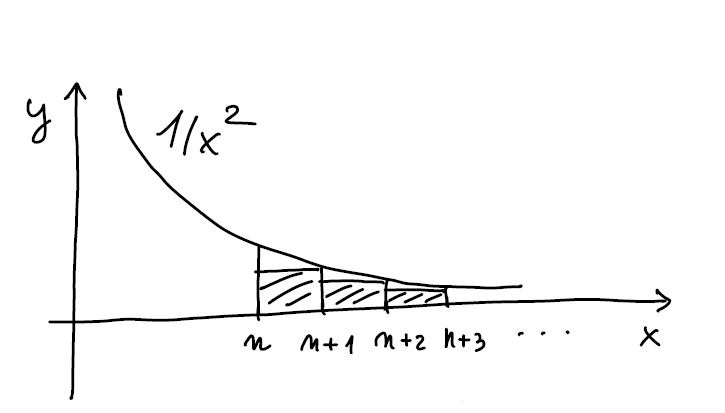
\includegraphics[width=0.6\textwidth]{pag24.jpg}
\end{center}
dove si vede che l'arco che sta sotto la curva $y=1/x^2$ tra $n$ e $\infty$ (cioè $\int_n^\infty \frac{1}{x^2}dx$) è maggiore della somma delle aree dei rettangolini che hanno base 1 e altezza $1/k^2$ con $k = n+1, n+2, \dotso$ cioè $\sum\limits_{k=n+1}^\infty \frac{1}{k^2}$. Quindi l'errore che si commette approssimando $\pi^2/6$ con $S_n$
si può stimare con $\frac{\pi^2}{6}-S_n < \frac{1}{n}$\\
Questo significa che per approssimare $\frac{\pi^2}{6}$ con un errore $<= \varepsilon_M$ (precisione di macchina) basta che $\frac{\pi^2}{6}-S_n < \frac{1}{n} <= \varepsilon_M$\\
cioè $n>=\varepsilon_M^{-1} \approx 10^{16}$, quindi bisognerebbe sommare $10^{16}$ (10 milioni di miliardi) di termini della serie!\\
D'altra parte in aritmetica di macchina ad un certo punto 
la somma $S_n$ diventerebbe costante, perché i termini che vanno sommati diventerebbero troppo piccoli e si comporterebbero come elementi neutri, impedendo di raggiungere la precisione richiesta (accade da $n\approx10^8$ in poi).\\ Considerando invece la successione definita "per ricorrenza" da\\\\
$x_0=2$\\
$x_{n+1}=2^{n-\frac{1}{2}}\cdot\sqrt{1-\sqrt{1-(4^{1-n})x_{n}^2}}$\\\\
$n=2,3,4,\dotso$\\
detta "successione di Archimede" si può dimostrare con metodi geometrici (legati all'approssimazione del cerchio con poligoni regolari) che $\lim\limits_{n\to\infty} x_n= \pi$. Se calcoliamo $x_n$ in Matlab con un semplice ciclo "for" e plottiamo l'errore relativo $r_n=\frac{|\tilde{x}_n-\pi|}{\pi}$ in SCALA LOGARITMICA , cioè plottiamo $log_{10}(r_n)$, otteniamo un grafico tipo quello disegnato di seguito in nero\\
\begin{center}
    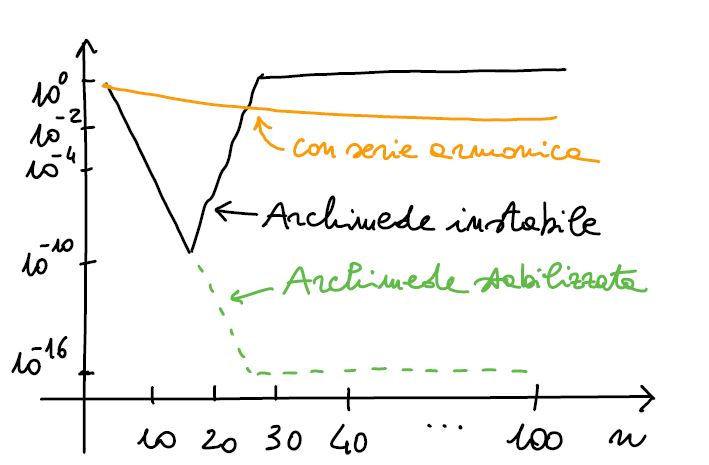
\includegraphics[width=0.5\textwidth]{pag28.JPG}
\end{center}
(dove abbiamo interpolato i valori discreti per una migliore visualizzazione). Si vede che l'errore decresce linearmente fino a circa $10^{-10}$ e poi comincia a crescere, cioè la successione $\tilde{x}_n$ calcolata
con lo schema descritto sopra in aritmetica di macchina da un certo n in poi comincia ad allontanarsi da $\pi$.\\
Si noti che fino a quel punto l'errore decade rapidamente, infatti un decadimento lineare in scala logaritmica significa che $log_{10}(r_n)=-\alpha n+\beta$ con $\alpha >0$ cioè in scala normale $r_n=10^{-\alpha n+\beta}=\delta\theta^n$ con $\delta=10^{\beta}$ e $\theta=10^{-\alpha}< 1$ che è un decadimento esponenziale (tanto più veloce quanto più grande è $\alpha$).\\
E' chiaro che l'algoritmo è instabile e che tale instabilità è in grado da un certo n in poi di distruggere la convergenza della successione (si osservi però che comunque la convergenza finchè c'è è rapida e permette di arrivare ad approssimare $\pi$ con un errore $\approx10^{-10}$ in meno di 20 iterazioni).\\ A cosa è dovuta l'instabilità? All'interno della radice quadrata esterna ci sono 2 sottrazioni, \\$1-\sqrt{1-\alpha_n}$, con $\alpha_n=4^{1-n}x^{2}_n$.\\
Visto che $\alpha_n$ è un infinitesimo, $\alpha_n \rightarrow0, n\rightarrow\infty$ (perchè $4^{-n}\rightarrow0$ e $x^{2}_n\rightarrow\pi^2, n\rightarrow\infty$) la sottrazione $1-\alpha_n$ è stabile (i numeri si allontanano in termini relativi al crescere di n).\\ Ma per lo stesso motivo la sottrazione $1-\sqrt{1-\alpha_n}$ diventa sempre più instabile al crescere di n, perchè $\sqrt{1-\alpha_n}\rightarrow1$,$n\rightarrow\infty$ e la convergenza a 1 è rapida ($|1-\sqrt{1-\alpha_n}|$ va a zero come $4^{-n}$). Possiamo calcolare il peso $w_2$ di questa sottrazione,
visto che $\sqrt{1-\alpha_n}$ è sicuramente affetto da errore (dell'ordine della precisione di macchina, visto che $\sqrt{}$ è una funzione predefinita calcolata alla precisione di macchina).\\ Posto $x=1, y=-\sqrt{1-\alpha_n}$ si ha\\
\begin{equation}
    \begin{split}
        w_2=\frac{|y|}{|x+y|}=\frac{\sqrt{1-\alpha_n}}{1-\sqrt{1-\alpha_n}}
        =\frac{\sqrt{1-\alpha_n}(1+\sqrt{1-\alpha_n})}{(1-\sqrt{1-\alpha_n})(1+\sqrt{1-\alpha_n})} \\
        =\frac{\sqrt{1-\alpha_n}(1+\sqrt{1-\alpha_n})}{\cancel{1}-(\cancel{1}-\alpha_n)}
        \approx\frac{2}{\alpha_n}=2\cdot\frac{4^{n-1}}{x^{2}_n}\approx\frac{1}{2\pi^2}4^n
    \end{split}
\end{equation}
Quindi il peso $ w_{2} $ è fattore di amplificazione che cresce esponenzialmente come $ 4^{n} $. Possiamo stimare l'errore $ e_{n}=\vert \pi-\widetilde{x_{n}}\vert $ in questo modo:
\begin{equation}
     e_{n}=\vert \pi - x_{n}+x_{x}-\widetilde{x_{n}}\vert \leq \vert \pi - x_{n}\vert + \vert x_{n}-\widetilde{x_{n}}\vert
\end{equation}
dove $ \vert \pi - x_{n}\vert$ è per la convergenza e $\vert x_{n}-\widetilde{x_{n}}\vert$ è per la stabilità, e dove l'errore $\vert \pi - x_{n} \vert $ è legato alla \underline{convergenza teorica} del metodo (in generale, dire che $ \lim\limits_{x\to \infty} x_{n} = l $ con $l$ limite finito è equivalente a dire che l'errore $ \vert x_{n} - l \vert \rightarrow 0, n \rightarrow \infty $), mentre l'errore $ \vert x_{n}-\widetilde{x_{n}}\vert $ è legato alla \underline{stabilità dell'algoritmo} che implementa il metodo. \\
Dall'analisi fatta, $\vert x_{n} - \pi \vert = c\theta^{n} $, con $0<\theta<1$ mentre $\vert \widetilde{x_{n}} - x_{n} \vert \lesssim c'4^{n}\varepsilon_{M}$ con c e c' costanti. Quindi 
\begin{equation}
     e_{n} \lesssim c\theta^{n} + c'4^{n}\varepsilon_{M}
\end{equation}
da cui ci aspettiamo che finché $c'4^{n}\varepsilon_{M}<c\theta^{n}$ si continui a vedere la convergenza, ma da quel punto in poi il termine esponenziale crescente comincia a sovrastare e in pratica fa allontanare la successione calcolata dal limite. \\
Si osservi che ad un certo punto l'errore diventa costante: questo accade quando $\alpha_{n}$ è così piccolo che $1\circleddash \alpha_{n} = 1$ e quindi $\widetilde{x_{n}}=0$ forzando un errore del 100\%.\\
È però possibile stabilizzare il calcolo di $x_{n}$ eliminando la sottrazione instabile, con lo stesso trucco utilizzato per le equazioni di $2^\circ$ grado. \\
Il cuore del problema è infatti il calcolo di  $1-\sqrt{1-\alpha_{n}}$ :
\begin{equation}
     1-\sqrt{1-\alpha_{n}}=\frac{(1-\sqrt{1-\alpha_{n}})(1+\sqrt{1-\alpha_{n}})}{1+\sqrt{1-\alpha_{n}}} = \frac{1-(1-\alpha_{n})}{1+\sqrt{1-\alpha_{n}}} = \frac{\alpha_{n}}{1+\sqrt{1-\alpha_{n}}}
\end{equation}
questa riscrittura è stabile in aritmetica floating-point, perchè sono coinvolte solo operazioni stabili.\\
Possiamo allora riscrivere l'iterazione in forma stabile 
\begin{equation}
     x_{n+1}=2^{n-\frac{1}{2}}\sqrt{1-\sqrt{1-\alpha_{n}}}=2^{n-\frac{1}{2}}\sqrt{\frac{\alpha_{n}}{1+\sqrt{1-\alpha_{n}}}}=\frac{\sqrt{2}x_{n}}{\sqrt{1+\sqrt{1-(4^{1-n})x_{n}^{2}}}}
\end{equation}
Nell'aritmetica dei reali le due formule sono coincidenti, mentre in aritmetica floating-point la seconda è stabile mentre la prima è fortemente instabile. Nel grafico degli errori in
scala logaritmica disegnato sopra, la successione stabilizzata
\begin{equation}
    y_{2}=2,   y_{n+1}=\frac{\sqrt{2}y_{n}}{\sqrt{1+\sqrt{1-4^{1-n}_{y_{n}^{2}}}}}, n\geq2
\end{equation}
calcolata in aritmetica di macchina, diciamola $\widetilde{y_{n}}$, fa un errore sostanzialmente coincidente con quello di $\widetilde{x_{n}}$ finché per quest'ultima si innesca l'instabilità, per poi continuare a diminuire secondo la stessa retta (cioè esponenzialmente in scala normale) fino ad attestarsi all'ordine della
precisione di macchina, di sotto alla quale ovviamente non si può andare in aritmetica di macchina, perché cominciano a dominare gli errori di arrotondamento, come si vede dalla stima
\begin{equation}
    \vert \pi - \widetilde{y_{n}} \vert \leq \vert \pi - y_{n} \vert + \vert y_{n} - \widetilde{y_{n}} \vert \lesssim c\theta^{n}+c''\varepsilon_{M} \text{ con } c''\approx \pi
\end{equation}
per n abbastanza grande \\ $c\theta^{n}\leq$c''$\varepsilon_{M}$ e quindi ci aspettiamo che il termine $c''\varepsilon_{M}$ diventi dominante nell'errore.
\end{document}
